\section{Руководство пользователя}

Разработанное програмное средство обладает интуитивно понятным интерфейсом и
привычными органами управления, характерными для большинства программ
мгновенного обмена сообщениями. При этом цветовая гамма и стиль элементов
управления выдержан в соответствии с оформлением социальной сети \vk{}.
 
При запуске программы осуществляется проверка наличия сохраненных данных об
авторизации. При отсутствии таких данных будет продемонстрировано окно
для проведения авторизации, изображенное на рисунке \ref{fig:vk_auth}.

\begin{figure}[h]
\centering
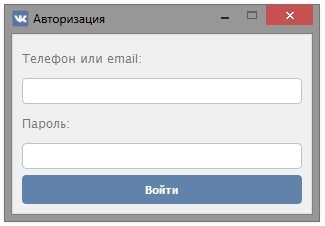
\includegraphics{vk_auth.jpg}
\caption{Окно авторизации пользователя}
\label{fig:vk_auth}
\end{figure}

В случае ошибки авторизации отобразится соответствующая информация. Пример
сообщения об ошибке предствлен на рисунке \ref{fig:vk_auth_error}.

\begin{figure}[h!]
\centering
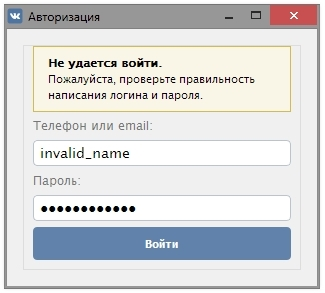
\includegraphics[scale = 0.9]{vk_auth_error.jpg}
\caption{Сообщение об ошибке авторизации}
\label{fig:vk_auth_error}
\end{figure}

После успешной авторизации произойдет открытие главного окна программы (рисунок
\ref{fig:vk_main}) и автоматическая синхронизация истории сообщений с данными
учётной записи \vk{}.

\begin{figure}[h] \centering 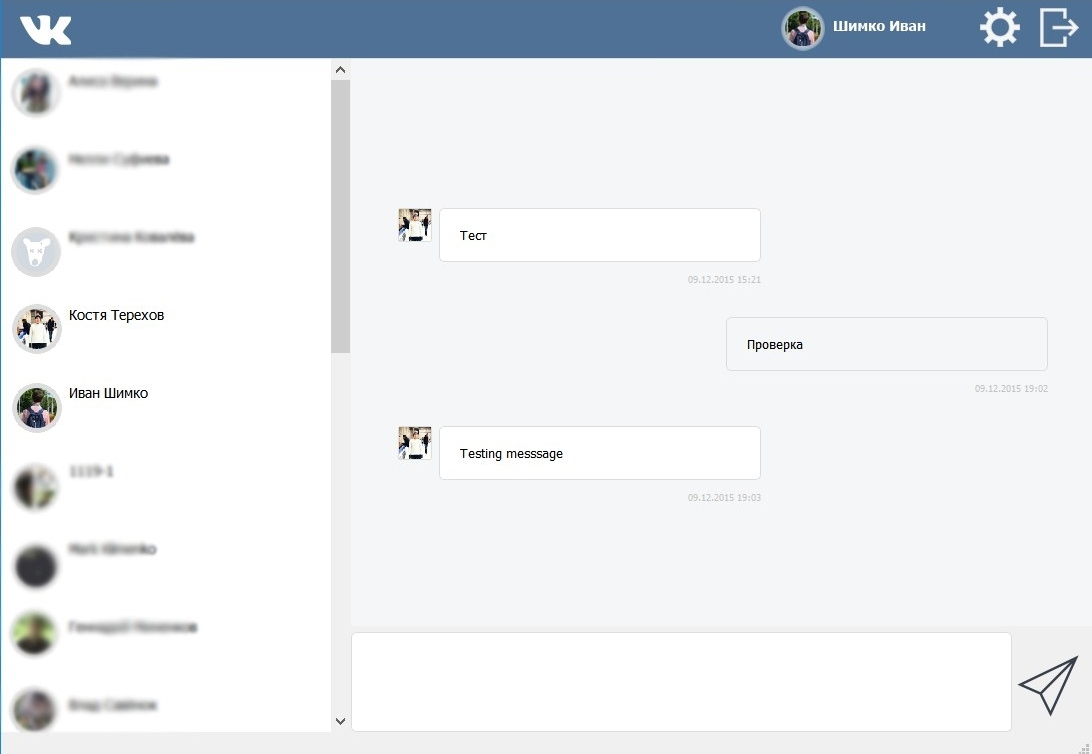
\includegraphics[scale = 0.3]{vk_main.jpg}
\caption{Главное окно \vkapp{}}
\label{fig:vk_main}
\end{figure}


В верхней панели программы находится информация об активной учётной записи,
кнопка для вызова меню настроек и кнопка выхода из приложения.

В левой части окна находится список активных диалогов пользователя,
отсортированный в порядке даты последнего сообщения. Выбор диалога
осуществляется простым кликом по соответствующему пункту списка.

После выбора нового диалога произойдёт запуск синхронизации данных кэша с
данными учётной записи.

В случае подозрительной активности со стороны учетной записи, серверы \vk могут
потребовать ввода кода с картинки. Пример окна для ввода данного кода приведено
на рисунке \ref{fig:vk_captcha}.

\begin{figure}[h]
\centering
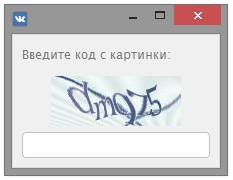
\includegraphics{vk_captcha.jpg}
\caption{Окно ввода капчи}
\label{fig:vk_captcha}
\end{figure}

Для отправки сообщения пользователю достаточно ввести сообщение в поле,
находящееся под историей сообщений и воспользоваться кнопкой с
соответствующей пиктограммой или сочетанием клавиш, выбранным в меню настроек.

Догрузка старых сообщений происходит автоматически при прокрутке истории
диалога.
Внешний вид меню настроек программы представлен на рисунке
\ref{fig:vk_settings}.

\begin{figure}[t]
\centering
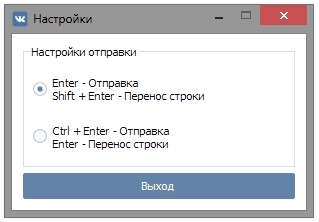
\includegraphics[scale = 0.9] {vk_settings.jpg}
\caption{Меню настроек}
\label{fig:vk_settings}
\end{figure}
Из данного меню возможно переключить настройки сочетаний клавиш для отправки
сообщения и переноса строки, а также осуществить выход из текущего аккаунта.

Выход из аккаунта приведет к очистке локального кэша и демонстрации окна для
повторного прохождения авторизации.
